\documentclass{report}
\usepackage{hyperref}
\usepackage[ngerman]{babel}
\usepackage{amsmath}
\usepackage{amsfonts}
\usepackage{amsthm}
\usepackage{tcolorbox}
\usepackage[a4paper, total={7in, 9in}]{geometry}
\usepackage[font={scriptsize,it}]{caption}
\usepackage{scrextend}
\usepackage{graphicx}
\usepackage{caption}
\usepackage{subcaption}
\usepackage[utf8]{inputenc}
\usepackage[T1]{fontenc}
\DeclareUnicodeCharacter{2212}{-}
\usepackage{verbatim}
\usepackage{tikz}

\tikzset{
  treenode/.style = {shape=rectangle, rounded corners,
                     draw, align=center,
                     top color=white, bottom color=blue!20},
  root/.style     = {treenode, font=\Large, bottom color=red!30},
  env/.style      = {treenode, font=\ttfamily\normalsize},
  dummy/.style    = {circle,draw}
}

\tikzstyle{level 1}=[level distance=3.5cm, sibling distance=3.5cm]
\tikzstyle{level 2}=[level distance=3.5cm, sibling distance=2cm]

% floating figure for column
\newenvironment{Figure}
	{\par\medskip\noindent\minipage{\linewidth}}
	{\endminipage\par\medskip}

\begin{document}

\begin{titlepage}
   \vspace*{\stretch{1.0}}
   \begin{center}
      \Large\textbf{eHealth Lab02 - HS20}\\
      \large\textit{Results from Pascal Brunner - brunnpa7}
   \end{center}
   \vspace*{\stretch{2.0}}
\end{titlepage}

% Beispiel Bild
%\begin{Figure}
%   \centering
%    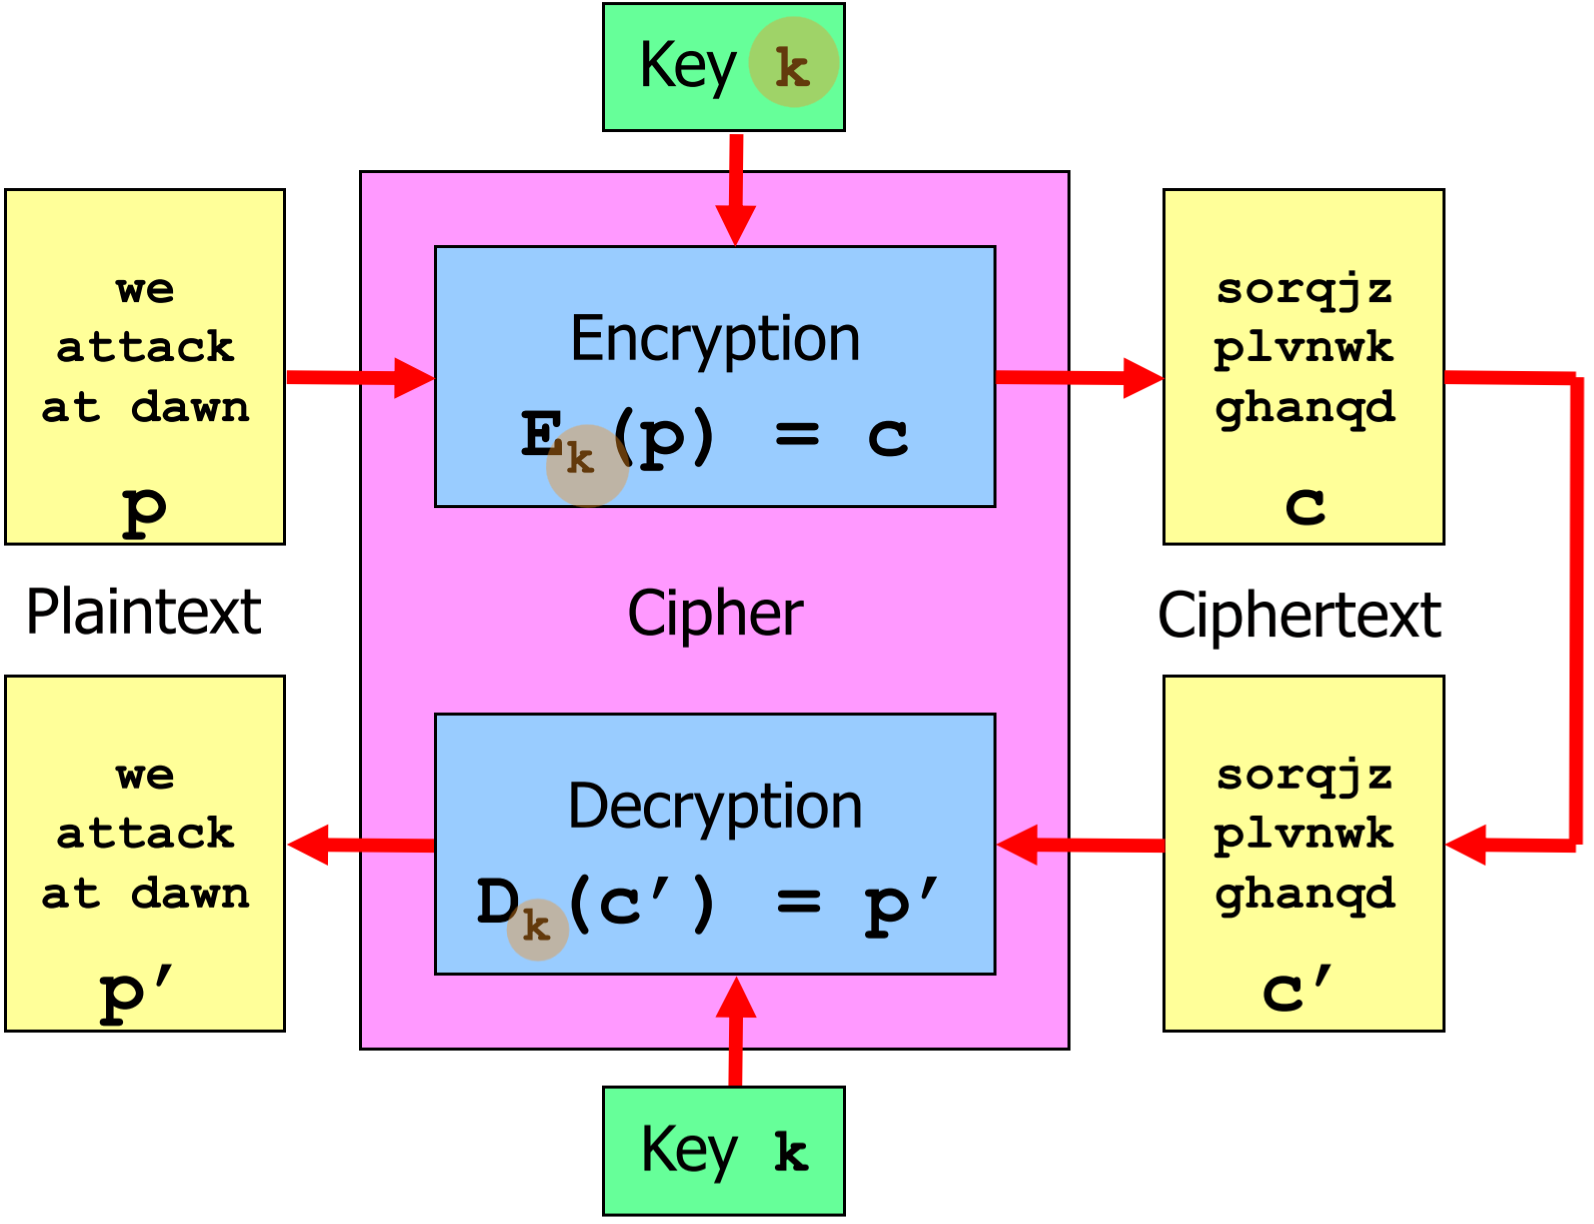
\includegraphics[width=150px]{img/BasicTerminologySecKeyCrypto.png}
%        \captionof{figure}{Basic Terminology basierend auf Secret Key Cryptography}
%        \label{fig:Basic Terminology}
%    \end{Figure}

\section*{Essay Lab 02}
\subsection*{current situation}
Since 15th of April 2017 exists the new \href{https://www.bag.admin.ch/bag/de/home/gesetze-und-bewilligungen/gesetzgebung/gesetzgebung-mensch-gesundheit/gesetzgebung-elektronisches-patientendossier.html}{law} 
about EHR in Switzerland. Hospitals must participate in the EHR and file the health information in the EHR, 
as must nursing homes from 2022 onwards. For all other treating persons, such as general practitioners, 
pharmacies or Spitex services, participation is voluntary. The EHR is also voluntary for citizens.
The hospitals had the deadline to implement the EHR in Q2 2020 - but this was not possible due to delays by the certification authority \href{https://www.e-health-suisse.ch/fileadmin/user_upload/Dokumente/D/factsheet-epd-einfuehrung.pdf}{newest factsheet (Juli 2020)}.
The introduction is iterative, i.e. from canton to canton. The introduction is also decentralized, through the various certification authorities. It is planned that the introduction will be completed by the end of Q1 2021 in each canton. 
A detailed rollout-plan can be viewed \href{https://www.e-health-suisse.ch/fileadmin/user_upload/Dokumente/D/einfuehrungsplan-epd-big-picture.pdf}{here}. \newline
\newline
Germany also aims to introduce it by January 2021. However, the health insurance companies are the driving force or the authority which is obliged to introduce this. 
But in Germany, too, the use of the system is voluntary for citizens. 
\newline
The situation is already different further north - in Denmark - where every inhabitant has received a so-called \href{https://www.handelskraft.com/digital-patient-records-the-danish-example/2019/03/}{NemID}. 
This ID enables every citizen to identify himself unambiguously in order to access official documents, for example. 
Not only can the most important official documents be accessed, but also the EHR can be managed. 
Thus, the citizen can grant access to family members, organ donation can be organized and manual information such as blood pressure 
can be entered directly.

\subsection*{evaluation of an EHR-System}
According to the factsheet, there are several main responsible authorities per canton:
\begin{itemize}
   \item \href{https://www.cara.ch/}{cara.} $\rightarrow$ FR, GE, JU, VD, VS
   \item \href{https://hesav.ch/dossier-sante/}{dossier santé} $\rightarrow$ NE
   \item \href{https://www.xsana.ch/bevoelkerung#benefits}{xsana} $\rightarrow$ BE, BL, BS, LU, NW, OW, SG, SH, SO, SZ, TG, UR, ZG, ZH
   \item \href{https://www.mein-emedo.ch/}{emedo} $\rightarrow$ AG 
   \item \href{https://www.ehti.ch/}{e-Health Ticino} $\rightarrow$ TI
   \item \href{https://esanita.ch/}{eSanita} $\rightarrow$ AI, AR, GL, GR, SG
   \item \href{https://www.abilis.ch/de}{abilis} $\rightarrow$ national, Switzerland
\end{itemize}

In Switzerland are two main EHR-Systems available. 
\begin{itemize}
   \item evita from Swisscom
   \item vivitas from Swiss Post
\end{itemize}

\subsection*{Evita from Swisscom}
I decided to sign up for the solution from Swisscom \textit{evita}. The whole process is really simple, I just had to confirm my mail and after that I can download some backup-SMS-Codes to restore my account.\\
After I confirmed my mail I filled out my personal information such as name, birthdate, address and so on. Once I completed my profile I have the opportunity to fill out or can connect a smartwatch for additional information about my health-status (see picture below):
\begin{Figure}
   \centering
    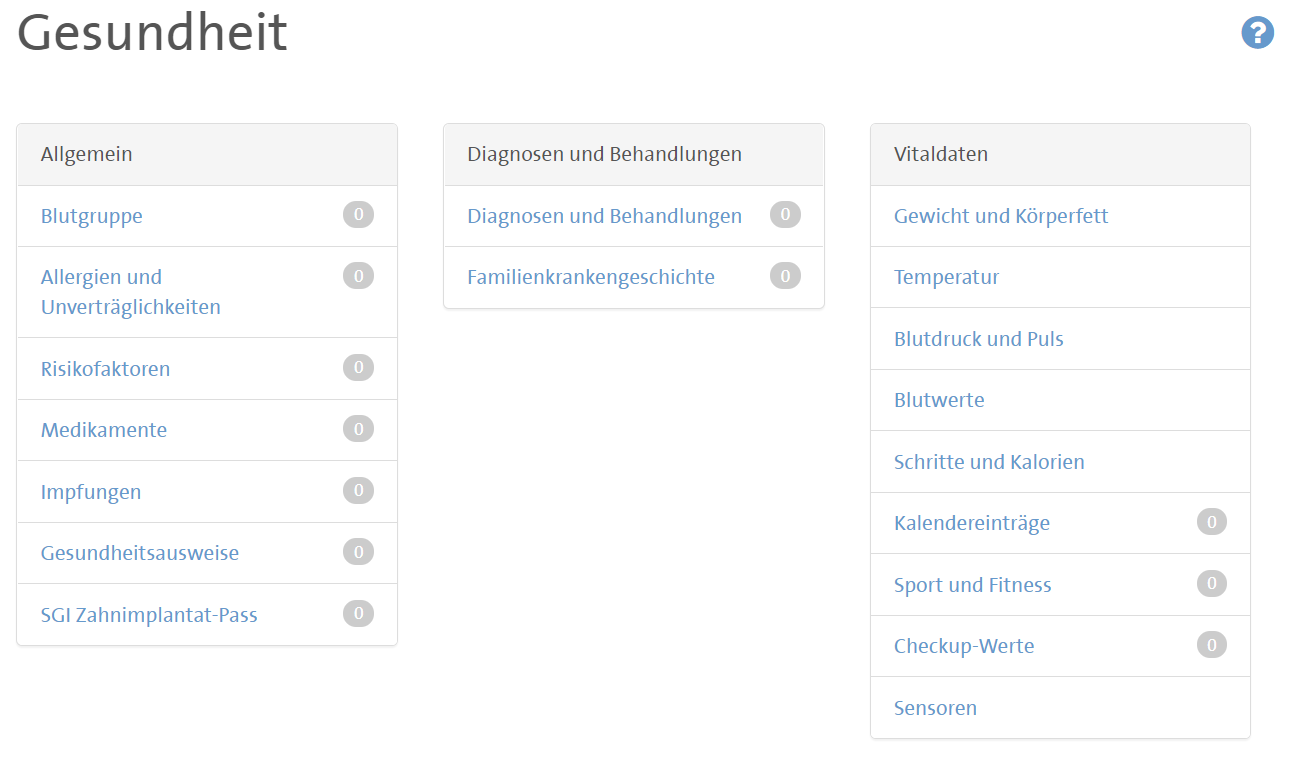
\includegraphics[width=250px]{img/Gesundheit.png}
        \captionof{figure}{List of additional information about the health-status}
        \label{fig:List of additional information about the health-status}
    \end{Figure}

In addition I have several information to fill out:
\begin{itemize}
   \item emergency contact
   \item general practitioner
   \item Medical document
   \item travel documents
   \item other documents
\end{itemize}

In the service-section are a lot of further services:
\begin{itemize}
   \item invoices
   \item Check-in for a stay at a hospital
   \item Docupass from pro Senctute
   \item Sign-up for eedoctors, which is a possibility to have a video-call with a doctor
\end{itemize}

Last but not least I can control the access to my EHR. I can add some additional person e.g. my family or girlfriend, but also my general practictioner as well as some organisations such as Spitex.\\
Unfortunately the general practictioner has to be partner of evita.
In this section it will be also shown if I have access to other dossiers e.g. for kids or something like that.\\
I am also aware that there is a "Log"-Part to see what is happening in my EHR.\\

\subsection*{Resumee}
In summary, it can be said that there are already some efforts in this area. However, there are current delays on the part of the federal government and the certification bodies that can be traced back. This has an overall effect on the whole process, which is why it is not yet live at the moment.\\
The EHR definitely has its advantages and will be indispensable in the future. I currently still see the difficulty when there are several providers and they are not connected. The goal should be that all doctors, hospitals and organizations are part of the system. \\
I personally will certainly use the EHR in the future as soon as 
\end{document}